%%%%%%%%%%%%%%%%%%%%%%%%%%%%%%%%%%%%%%%%%%%%%%%%%%%%%%%%%%%%%%%%%%%%%%
% Template modified by Fernando Paolo from:
%
% LaTeX Template: Designer's CV
%
% Source: http://www.howtotex.com
%
% Feel free to distribute this example, but please keep the referral
% to HowToTeX.com
%
% Date: March 2012
%
% Modified by Lim Lian Tze to support multiple pages using fix provided at
% http://www.howtotex.com/templates/creating-a-designers-cv-in-latex/
% Date: November 2014
%
% Modified by Fernando Paolo to fit more information by changing the
% page layout (white space and column sizes).
% Data: September 2015
%
% To compile simply run:
%
% pdflatex source.tex
%%%%%%%%%%%%%%%%%%%%%%%%%%%%%%%%%%%%%%%%%%%%%%%%%%%%%%%%%%%%%%%%%%%%%%

%%%%%%%%%%%%%%%%%%%%%%%%%%%%%%%%%%%%%
% Document properties and packages
%%%%%%%%%%%%%%%%%%%%%%%%%%%%%%%%%%%%%
\documentclass[a4paper,11pt,final]{memoir}

% misc
\renewcommand{\familydefault}{bch}  % font
\pagestyle{empty}                   % no pagenumbering
\setlength{\parindent}{0pt}         % no paragraph indentation

% required packages (add your own)
\usepackage{flowfram}                                       % column layout
\usepackage[top=1cm,left=1cm,right=1cm,bottom=1cm]{geometry}% margins
\usepackage{graphicx}                                       % figures
\usepackage{url}                                            % URLs
\usepackage[usenames,dvipsnames]{xcolor}                    % color
\usepackage{multicol}                                       % columns env.
    \setlength{\multicolsep}{0pt}
\usepackage{paralist}                                       % compact lists
\usepackage{tikz}
\usepackage[nodayofweek]{datetime}
\usepackage{hyperref}

% customize date
\newdateformat{mydate}{\twodigit{\THEDAY}{ }\shortmonthname[\THEMONTH], \THEYEAR}

%%%%%%%%%%%%%%%%%%%%%%%%%%%%%%%%%%%%%
% Create column layout
%%%%%%%%%%%%%%%%%%%%%%%%%%%%%%%%%%%%%
% define length commands
\setlength{\vcolumnsep}{\baselineskip}
\setlength{\columnsep}{\vcolumnsep}

% left frame
\newflowframe{0.16\textwidth}{\textheight}{0pt}{0pt}[left]
    \newlength{\LeftMainSep}
    \setlength{\LeftMainSep}{0.18\textwidth}
    \addtolength{\LeftMainSep}{0.75\columnsep}

% small static frame for the vertical line
\newstaticframe{1.5pt}{\textheight}{\LeftMainSep}{0pt}

% content of the static frame
\begin{staticcontents}{1}
\hfill
\tikz{%
    \draw[loosely dotted,color=NavyBlue,line width=2.pt,yshift=0]
    (0,0) -- (0,\textheight);}
\hfill\mbox{}
\end{staticcontents}

% right frame
\addtolength{\LeftMainSep}{1.5pt}
\addtolength{\LeftMainSep}{1\columnsep}
\newflowframe{0.75\textwidth}{\textheight}{\LeftMainSep}{0pt}[main01]


%%%%%%%%%%%%%%%%%%%%%%%%%%%%%%%%%%%%%
% define macros (for convience)
%%%%%%%%%%%%%%%%%%%%%%%%%%%%%%%%%%%%%
\newcommand{\Sep}{\vspace{1.25em}}
\newcommand{\SmallSep}{\vspace{0.5em}}

\newenvironment{Research}
    {\ignorespaces\textbf{\color{NavyBlue} Research}}

\newcommand{\CVSection}[1]
    {\Large\textbf{#1}\par
    \SmallSep\normalsize\normalfont}

\newcommand{\CVItem}[1]
    {\textbf{\color{NavyBlue} #1}}

%%%%%%%%%%%%%%%%%%%%%%%%%%%%%%%%%%%%%
% Begin document
%%%%%%%%%%%%%%%%%%%%%%%%%%%%%%%%%%%%%
\begin{document}

% Left frame
%%%%%%%%%%%%%%%%%%%%
%
% Upload your own photo using the files menu
%\begin{figure}
%    \hfill
%    \includegraphics[width=0.6\columnwidth]{cv-photo.png}
%    \vspace{-7cm}
%\end{figure}

\begin{flushright}\small
    crocha@ucsd.edu\\[.1cm]
    crocha700.github.io\\[.1cm]
    github: crocha700\\[.1cm]
    vimeo: crocha700\\[.1cm]
    ORCID: 0000-0003-4063-5468\\[.1cm]
    \textcolor[gray]{0.45}{\mydate\today}\\[.1cm]
    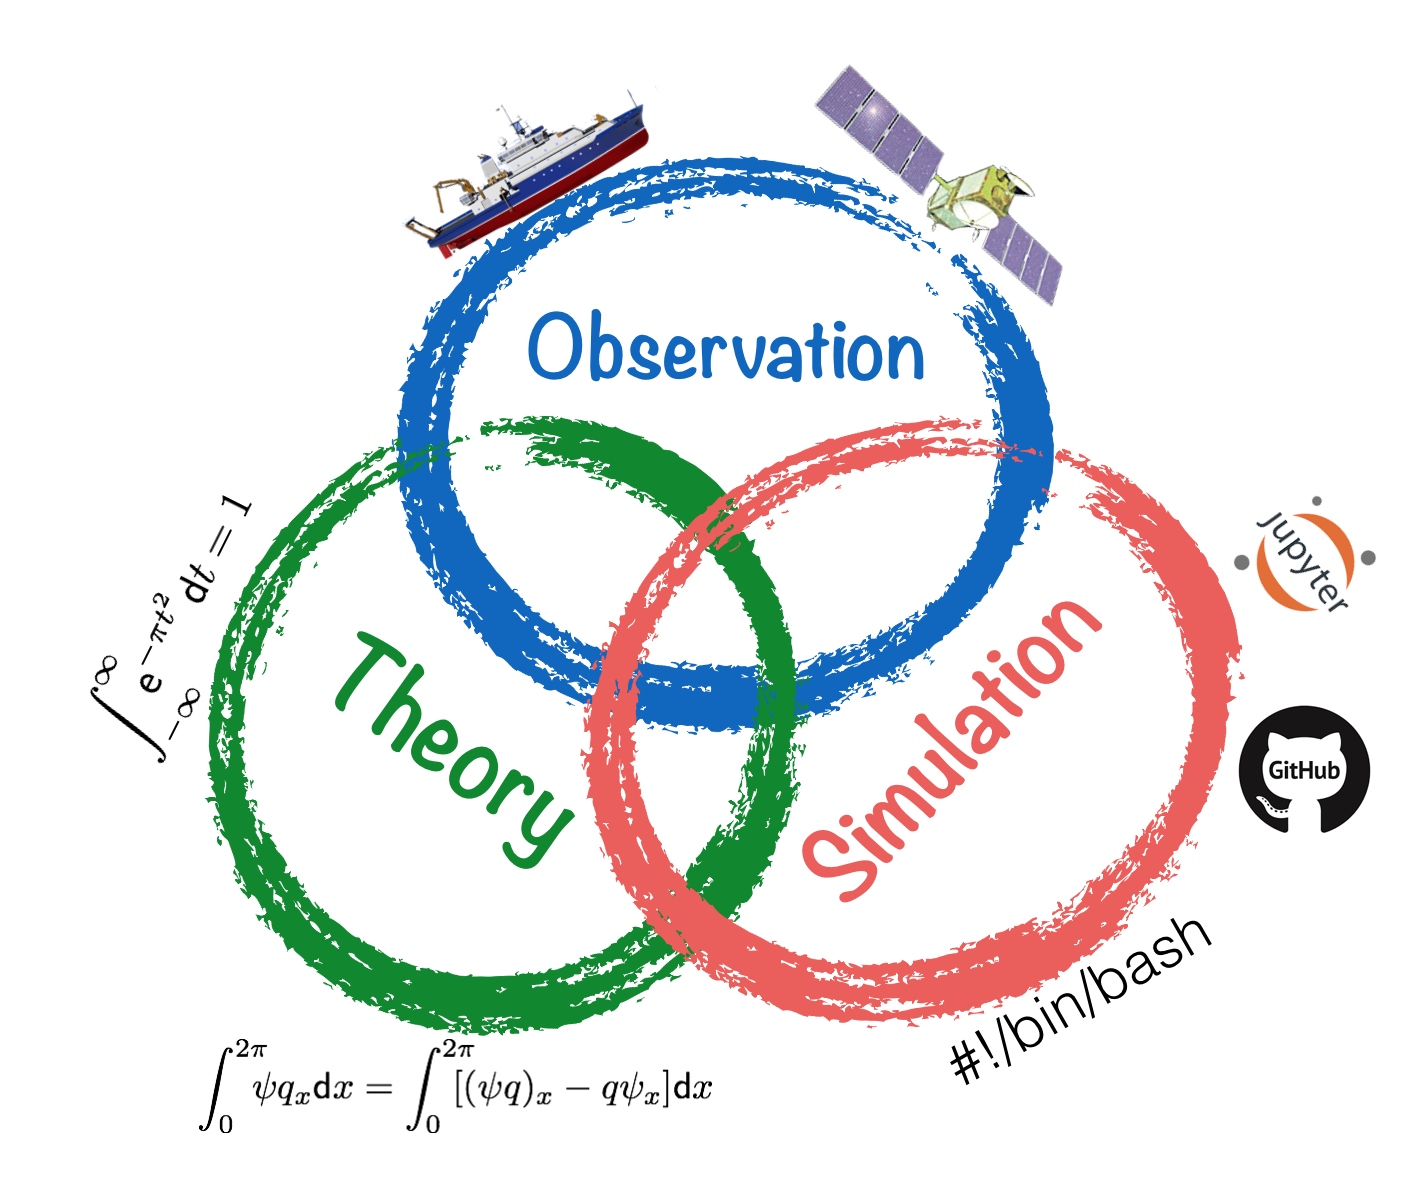
\includegraphics[width=.185\textwidth]{theory_comp_obs2.png}
\end{flushright}\normalsize
\framebreak

% Right frame
%%%%%%%%%%%%%%%%%%%%
\Huge\bfseries { \color{NavyBlue}  Cesar B Rocha} \\
\Large\bfseries Physical oceanographer \\

\normalsize\normalfont

%%% About me
\begin{Research}
I combine theory, computer simulations, and observations to study how the ocean flows and shapes the climate.
My motivation stems from genuine curiosity and awe at the ocean and the societal relevance
of oceanography in the anthropocene. Lately, my research efforts have
targeted the turbulent and wavy dynamics of the upper ocean at horizontal scales between 1-300 km.

\end{Research}

\Sep

%%% Education
\CVSection{Education}

Ongoing, PhD in Oceanography, University of California, San Diego \\
BSc, MSc in Oceanography, University of S\~ao Paulo, Brazil (\textit{summa cum laude}) \\

\Sep

%%% Experience
\CVSection{Experience}

\CVItem{2015, Fellow in Geophysical Fluid Dynamics, GFD Program, WHOI}\\
Coupled reduced equations for strongly stratified flows.
\SmallSep

\CVItem{2013--Current, Graduate Student Researcher, SIO/UCSD}\\
Stratified planetary turbulence and dynamics of the upper ocean.
\SmallSep

\CVItem{2012, Visiting student, University of Massachusetts Dartmouth}\\
Quasigeostrophic modes and surface quasigeostrophic solutions.
\SmallSep

\CVItem{2011--2013, Master Student, University of Sao Paulo}\\
Energetics and dynamics of the Brazil Current System.


\Sep

\CVSection{Publications}

\CVItem{Submitted }\\

%3. \textbf{Rocha, C. B.} and W. R. Young: Homogeneous quasigeostrophic turbulence driven by uniform wind stress, to be submitted to JFM.
%\SmallSep

2. Ardhuin, F., Gille, S., Menemenlis, D., \textbf{Rocha, C. B.}, Rascle, N., Chapron, B., Gula, J., Molemaker, J.: Small scale currents have large effects on ocean wave heights, under review for JGR-Oceans.

\SmallSep

\CVItem{Peer-reviewed}\\

5.  \textbf{Rocha, C. B.},  Gille, S. T., Chereskin, T. K., and Menemenlis, D.: Seasonality of submesoscale dynamics in the Kuroshio Extension, \textit{Geophys. Res. Lett.}, \textit{in press},
doi: 10.1002/2016GL071349.

\SmallSep

4.\,\textbf{Rocha, C. B.};  Chereskin, T. K.; Gille, S. T. and Menemenlis, D., 2016: ``Mesoscale to submesoscale wavenumber spectra in Drake Passage'', \textit{J. Phys. Oceanogr.}, 46 (2), 601-620, doi:10.1175/JPO-D-15-0087.1.

\SmallSep

3.\,\textbf{Rocha, C. B.};  Young, W. R. and Grooms, I., 2016: ``On Galerkin approximations of the surface-active quasi-geostrophic equations'', \textit{J. Phys. Oceanogr.}, 46 (1), 125-139, \texttt{doi:10.1175/JPO-D-15-0073.1}

\SmallSep

2.\,\textbf{Rocha, C. B.};  da Silveira, I. C. A., Castro, B. ,M. and Lima, J. A. M., \textbf{2014}: ``Vertical structure, energetics and dynamics of the Brazil Current System at 22$^\circ$S-28$^\circ$S'', \textit{ J. Geophys. Res., 119,} \href{http://onlinelibrary.wiley.com/doi/10.1002/2013JC009143/abstract}{\texttt{doi:10.1002/2013JC009143}.}

\SmallSep

1.\,\textbf{Rocha, C. B.}; Tandon, A.; da Silveira, I. C. A. and Lima, J. A. M., \textbf{2013}: ``Traditional Quasi-geostrophic modes and Surface Quasi-geostrophic solutions in the Southwestern Atlantic'', \textit{ J. Geophys. Res., 118 (5),} \href{http://dx.doi.org/10.1002/jgrc.20214}{\texttt{doi:10.1002/jgrc.20214}.}

\SmallSep

\clearpage
\framebreak
\framebreak


\CVItem{Grey literature}\\

1.\, \textbf{Rocha, C. B.}, 2015: Coupled reduced equations for strongly stratified flows,  Proceedings of the Geophysical Fluid Dynamics Program,  Woods Hole Oceanographic Institution, Woods Hole, MA.

\Sep

\CVSection{Invited Seminars}

1. Oceans and Cryosphere Seminar Series, Jet Propulsion Laboratory, Fall 2015

\Sep

\CVSection{Software}

3.\, Core developer for ``Python quasigeostrophic model'' (PyQG),

\href{http://dx.doi.org/10.5281/zenodo.30517}{\texttt{doi.org/10.5281/zenodo.30517}}

\SmallSep

2.\, Core developer for ``Spectral Analysis in Python'' (PySpec),

\href{http://dx.doi.org/10.5281/zenodo.31596}{\texttt{doi.org/10.5281/zenodo.31596}}

1.\, Contributor to a number of open source projects on github.

\Sep


\CVSection{Service}


Ongoing: Reviewer for Deep Sea Research-I, Geophysical Research Letters, Journal of
        Fluid Mechanics, Nature Communications, Ocean Modelling. \\

2016: Member of student committee as part of the
SIO faculty search in large scale observational physical oceanography.\\

2015-2016: Mentor for 1st yr SIO Graduate Students. \\

2015: Member of student committee for the SIO teaching award.




%2015, Reviewer for JGR-Oceans, JPO, GRL, Nature, Science, NSF, NASA

\Sep

\CVSection{Honors \& Awards}
2016, NASA Earth \& Space Science Graduate Fellowship\\
2015, Geophysical Fluid Dynamics Fellowship, Woods Hole Oceanographic Institution\\
2011, Best BSc thesis in Oceanography, University of Sao Paulo

\Sep

%%% Skills
\CVSection{Skills}

\CVItem{Programming}\\
Python , C, Fortran 90, Shell-Script, Matlab, git, mercurial, markdown

\SmallSep

\CVItem{Languages}\\
English (fluent), Portuguese (native), Spanish (professional fluency)

\Sep

%%% Skills
\CVSection{Membership}

%Golden Key International Honour Society, American Geophysical Union, The Oceanography Society, NumFOCUS (open code, better science)
 American Geophysical Union, The Oceanography Society, NumFOCUS

\Sep

%%% other
\CVSection{Other interests}

Data science, Scientific reproducibility, Free software, Open science, History and philosophy of science

%\Sep
%
%\CVSection{References}
%
%\CVItem{William R. Young}\\
%Distinguished Professor of Oceanography, UC San Diego, \texttt{wryoung@ucsd.edu}
%
%\SmallSep
%
%\CVItem{Sarah T. Gille}\\
%Professor of Oceanography, UC San Diego, \texttt{sgille@ucsd.edu}
%
%\SmallSep
%
%\CVItem{Teresa K. Chereskin}\\
%Research Oceanographer and Senior Lecturer, UC San Diego, \texttt{tchereskin@ucsd.edu}
%
%\SmallSep
%
%\CVItem{Myrl Hendershott}\\
%Professor of Oceanography, UC San Diego, \texttt{mch@ucsd.edu}


%\SmallSep

%\CVItem{Dimitris Menemenlis}\\
%Research Scientist, JPL/NASA, \texttt{dimitris.menemenlis@jpl.nasa.gov}








%% You'll need these 3 lines at the end of each page!
%\clearpage
%\framebreak
%\framebreak
%
%(\emph{Honors \& Awards continued})\\
%2007--2008, Brazilian Ministry of Sci. \& Tech. Fellowship (Masters)\\
%2007, Honor Mention (2nd best BSc Thesis), University of S\~ao Paulo\\
%2005--2006, S\~ao Paulo Research Foundation Fellowship (Undergrad)\\
%2004, Brazilian Ministry of Sci. \& Tech. Fellowship (Undergrad)
%
%\Sep
%
%\CVSection{Teaching}
%Aug--Dec 2008, Computing for Geophysicists, T.A. at University of S\~ao Paulo\\
%Mar--Jul 2008, Introduction to Geophysics, T.A. at University of S\~ao Paulo
%
%\Sep
%
%\CVSection{Fieldwork}
%Dec 2004, Geophysical and Geological Survey, SE Brazil (12 days at sea)\\
%Jan 2004, Brazilian Antarctic Research Station (30 days in Antarctica)\\
%Dec 2003, Environmental Monitoring Program, NE Brazil (14 days at sea)\\
%Jan 2003, Oceanographic Moorings II, SE Brazil (8 days at sea)\\
%Jul 2002, Oceanographic Moorings I, SE Brazil (9 days at sea)




%% You'll need these 3 lines at the end of each page!
%\clearpage
%\framebreak
%\framebreak
%
%\CVItem{2005 - 2007, Vivamus vel bibendum}\\
%Proin rutrum pharetra molestie. Cras sollicitudin nulla nec leo lobortis in tristique purus pretium. Ut eu felis nulla.
%\Sep
%
%
%% Skills
%\CVSection{Skills}
%\CVItem{Platforms}
%\begin{multicols}{3}
%\begin{compactitem}[\color{NavyBlue}$\circ$]
%    \item Lorem
%    \item Ipsum
%\end{compactitem}
%\end{multicols}
%\SmallSep
%
%\CVItem{Computer software}
%\begin{multicols}{3}
%\begin{compactitem}[\color{NavyBlue}$\circ$]
%    \item Lorem
%    \item Ipsum
%    \item Dolor
%    \item Sit
%    \item Amet
%    \item Consectetur
%    \item Adipiscing
%    \item Elit
%    \item \ldots
%\end{compactitem}
%\end{multicols}
%\Sep
%
%% References
%\CVSection{References}
%References upon request.

%%%%%%%%%%%%%%%%%%%%%%%%%%%%%%%%%%%%%
% End document
%%%%%%%%%%%%%%%%%%%%%%%%%%%%%%%%%%%%%
\end{document}
